
In this chapter, we will present and formalize the key properties of planar graph regions that will be exploited in the following chapter. We will also describe efficient methods for obtaining such a division.

\begin{defn} [$r$-division \cite{frederickson}]
\label{$r$-division}
We call \emph{r-division} a graph division into $\Theta(n/r)$ regions of $O(r)$ vertices each and $O(\sqrt{r})$ boundary vertices each.
\end{defn}

This definition only restricts the graph division in terms of region size and number of boundary vertices, but these criteria do not guarantee a desirable structure for the regions. There are two main issues with defining division in this way. Firstly, a single boundary vertex may be shared by more regions than its degree. Secondly, a single region might consist of multiple disconnected parts scattered throughout the entire graph. To not lose the benefits of graph planarity we introduce stricter definition of graph division.

\begin{defn} [suitable $r$-division \cite{frederickson}]
\label{suitable}
A \emph{suitable r-division} of a planar graph is an $r$-division that also satisfies:
\begin{itemize}
    \item every boundary node is at most in three different regions,
    \item every region is either connected component or union of connected components that share boundary nodes with the same set of either one or two regions that are connected components (see \Cref{fig:suitableExample}).
\end{itemize}
\end{defn}

\begin{figure}[H]
    \centering
        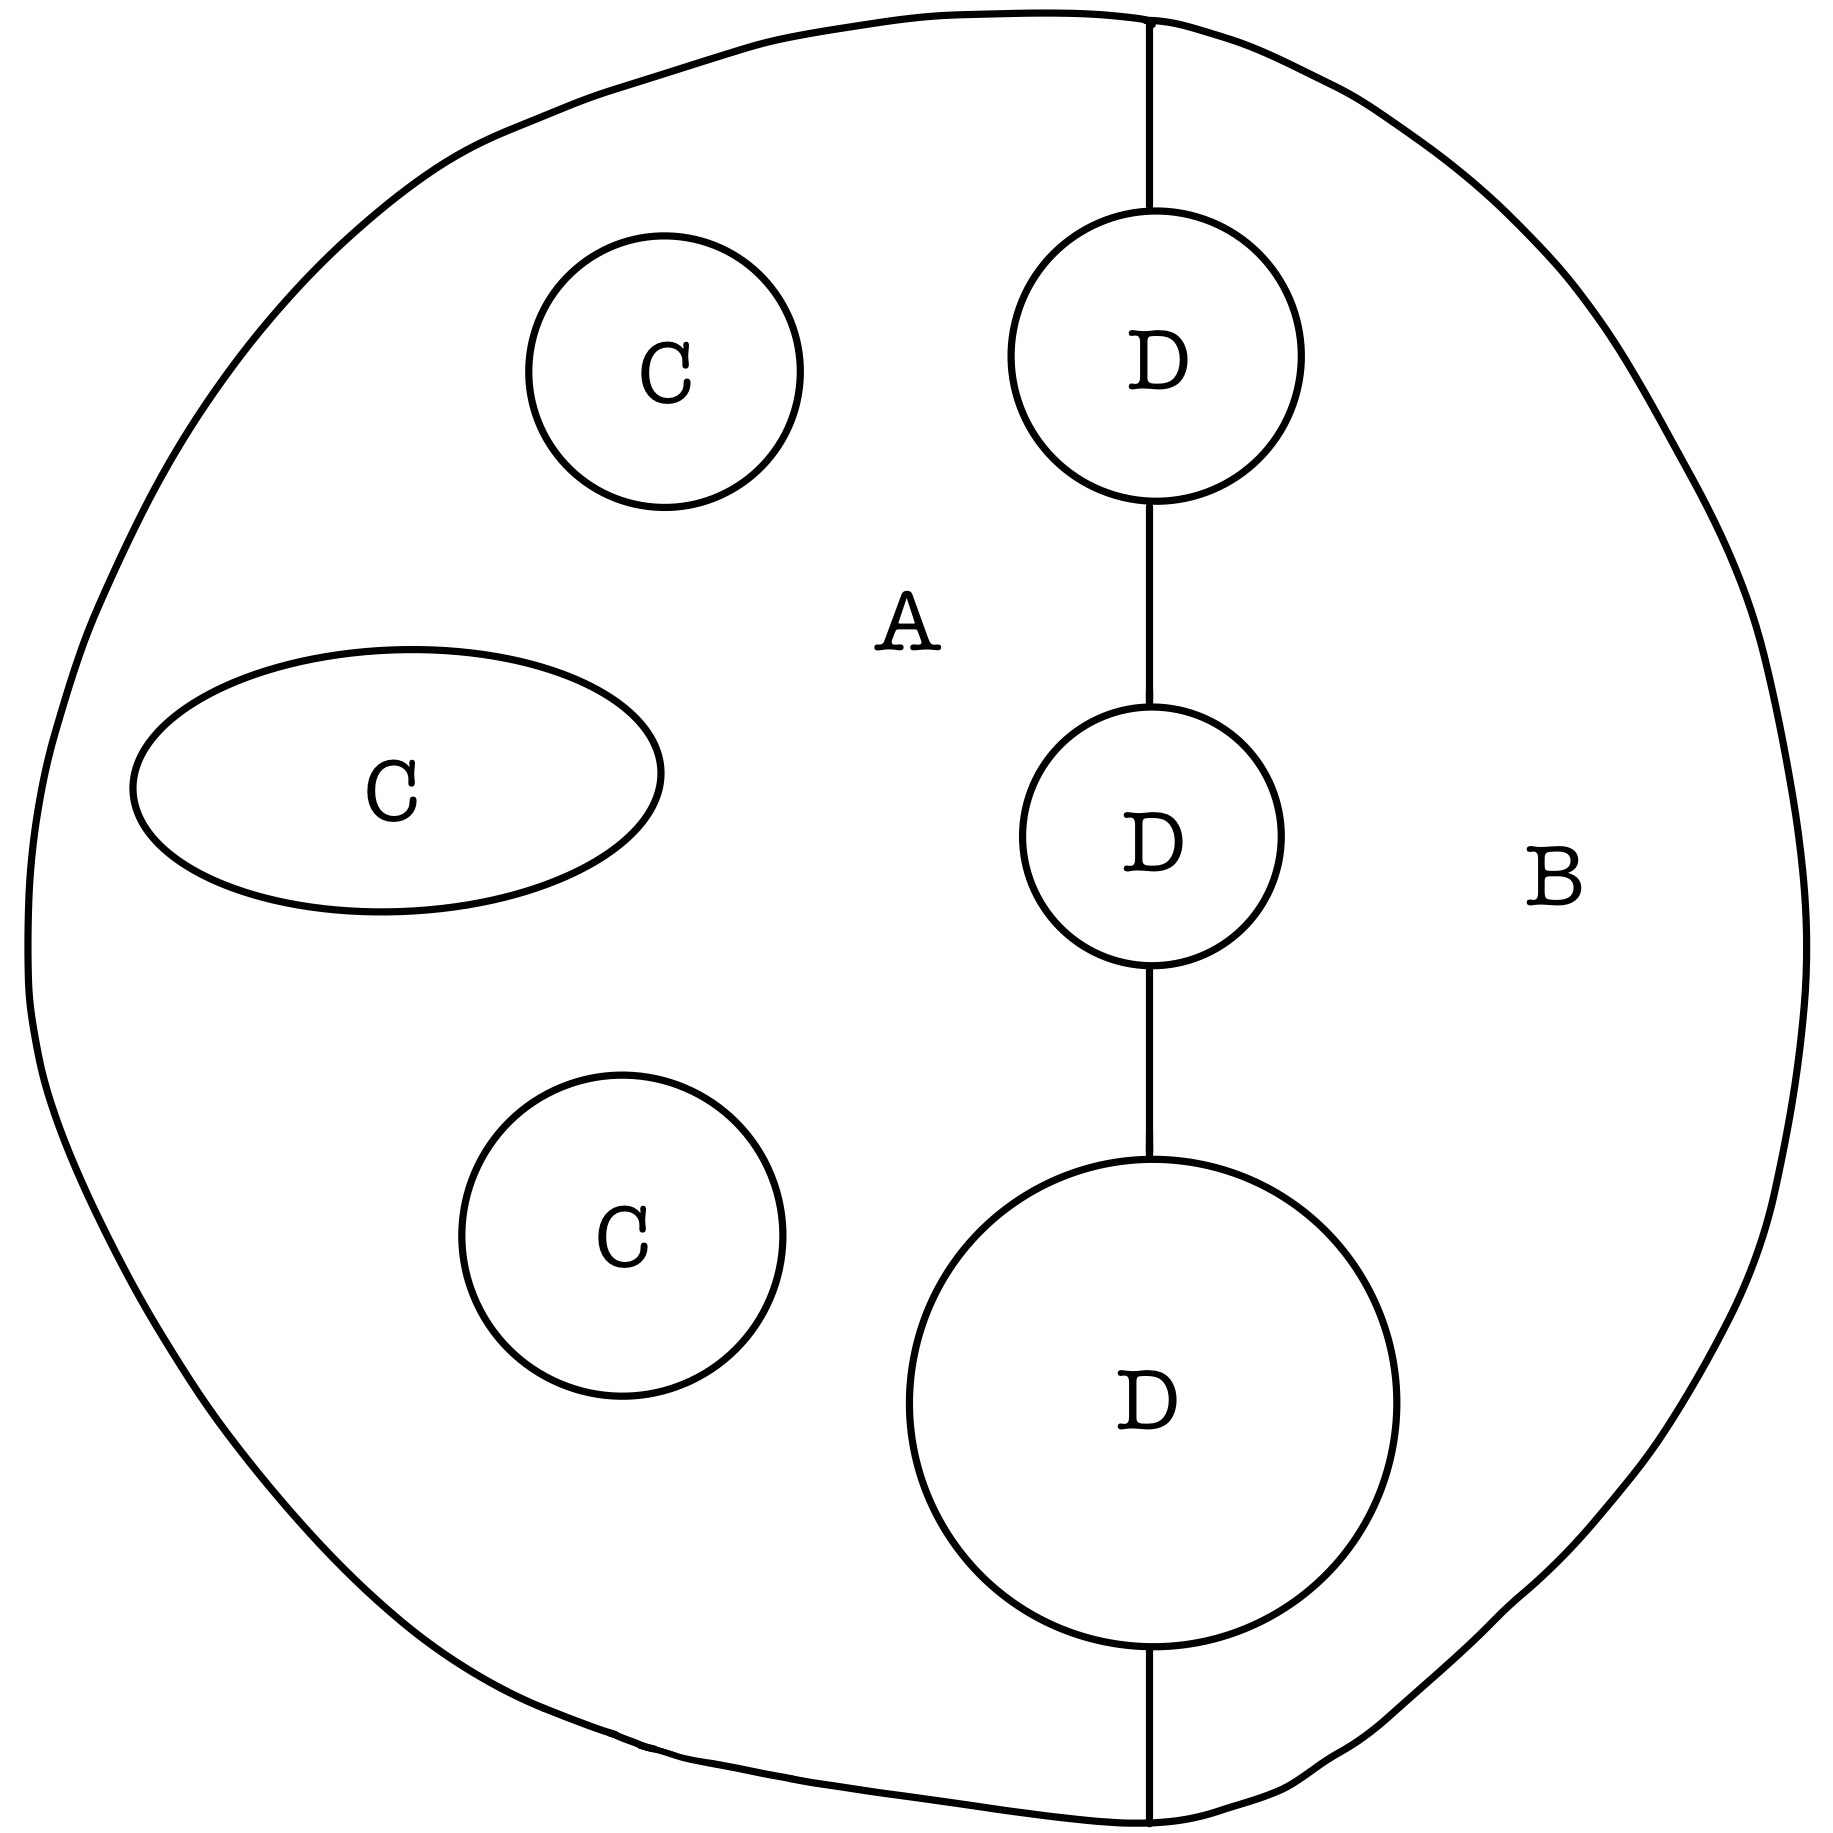
\includegraphics[width=0.6\textwidth]{2-Graph_Division/assets/IMG_8196.JPG}
    \caption{Examples of regions that are unions of connected components \cite{frederickson}.}
    \label{fig:suitableExample}
\end{figure}

\section{Recursive division}
% $2/3$, $2\sqrt{2n}$
To find $r$-division implementation of Planar Separator Theorem \cite{separatorT} will be used. The separator algorithm given graph $G$ with weighted vertices, partitions the vertices of $G$ into three sets $A$, $B$ and $C$ (the separator). The partition is such that no edge joins a vertex in set $A$ with a vertex in set $B$. Moreover the sum of weights in sets $A$ and $B$ does not exceed $2/3$ of the sum of weights in the entire graph. Algorithm also ensures that set $C$ is small, i.e. it does not contain more than $O(\sqrt{n})$ vertices. For the purpose of this analysis if not stated differently the nodes will have equal weight. This means that the sum of weights can be treated as number of vertices in a given set.

There are several known implementations of the Planar Separator algorithm, each providing different constants for the separator size. For the purposes of this work, it suffices to use any separator of size $O(\sqrt{n})$. However, for completeness, we present some of these variants below.

\begin{table}[h!]
\centering
\begin{tabular}{|c|c|c|}
\hline
Algorithm & Separator size & Time \\
\hline
Lipton, Tarjan \cite{separatorT} & $\leq 2\sqrt{2n} = 2.83 \sqrt{n}$ & $O(n)$\\
\hline
Alon, Seymour and Thomas \cite{secondBestSeparator} &  $ \leq 2.13\sqrt{n}$ & $O(n)$ \\
\hline
Djidjev and Venkatesan \cite{Djiev} & $ \leq 1.97\sqrt{n}$ & $O(n)$ \\
\hline
Fundamental Cycle Separator \cite{separatoPrzeglad} & $O(d)$ $d$ is diameter of a graph & $O(n)$\\
\hline
\end{tabular}
\caption{Example of planar separator implementations}
\label{tab:przyklad}
\end{table}

The best known lower bound for the size of a planar separator is $1.55\sqrt{n}$~\cite{separatorBound}. Although the separator size produced by the Fundamental Cycle Separator algorithm can be as large as $O(n)$ in the worst case, this approach performs very well in practice and is easy to implement, which is why it is often chosen in practical applications.

Our algorithm computing $r$-division consists of two parts. The first part starts by obtaining a planar graph division with $O(n/r)$ regions of size $O(r)$ and in total $O(n/\sqrt{r})$ boundary vertices using \Cref{firstPart}. The second part builds on top of that further dividing regions ensuring appropriate number of boundary vertices per region.
\begin{algorithm}
\caption{\textsc{RecursivePartition}}\label{firstPart}
\begin{algorithmic}[1]
\Require Planar graph $G = (V, E)$, region size parameter $r$
\Ensure Partition of $G$ into regions of size at most $r$
\Procedure{RecursivePartition}{$G$, $r$}
    \State  $R \gets \{V\}$
    \While{ exists $S \in R$ that $|S| \geq r$}
        \State $R \gets R \setminus \{S\}$
        \State $A,B,C \gets$ \Call{Separator}{$G[S]$}
        \State $R \gets R \cup \{A \cup C, B \cup C\}$
    \EndWhile
    \State \Return $R$
\EndProcedure

\end{algorithmic}
\end{algorithm}

\begin{lemma}[Lemma 1 in \cite{frederickson}]
    The planar graph on $n$ vertices can be divided into $O(n/r)$ regions of size $O(r)$ with $O(n/\sqrt{r})$ boundary vertices in $O(n \log{n/r})$.
\end{lemma}

\begin{proof}
The time complexity claim can be proven by analyzing the recursion tree of \Cref{firstPart}. Since the recursion stops when regions reach size $O(r)$, the process terminates $\log r$ levels before reaching the leaves. As a result, the recursion tree has $\log n - \log r = \log(n/r)$ levels, each requiring $O(n)$ work.
It is obvious that procedure described above will create $O(n/r)$ regions of size $O(r)$. We need to now prove that the number of boundary nodes is appropriate.
By $b(v)$ we will denote one less than the number of regions that $v$ is contained. Let $B(n,r) = \sum_{v \in V} b(v)$. Intuitively, we can treat $B(n,r)$ as number of copies of all boundary vertices in a division. By applying bounds for resulting sets size and number of boundary vertices we get the following recurrence:

\begin{align*}
B(n,r) \leq 2 \sqrt{2n} + B(\alpha n + O(\sqrt{n}), r) + B((1-\alpha)n + O(\sqrt{n}), r)& \text{  for $n > r$},\\
B(n,r) = 0 & \text{ for $n \leq r$},
\end{align*}
where $1/3 \leq \alpha \leq 2/3$. Intuitively, the number of new copies in a division is bounded both by the separator size and subsequent copies added by recursive divisions.

We will prove by induction that for some constant $d > 0$ it holds that:
$$B(n,r) \leq 2\sqrt{2}\frac{n}{\sqrt{r}} - d\sqrt{n}.$$
    

By applying the inductive step and summing up, we get:
\begin{align*}
B(n, r) &\leq 2\sqrt{2n} + 2\sqrt{2}\frac{\alpha n}{\sqrt{r}} + 2\sqrt{2}\frac{(1-\alpha) n}{\sqrt{r}} + O\left(\frac{\sqrt{n}}{\sqrt{r}}\right) - d(\sqrt{\alpha n} + \sqrt{(1-\alpha)n}) \\
&= 2\sqrt{2n} + 2\sqrt{2}\frac{n}{\sqrt{r}} + O\left(\frac{\sqrt{n}}{\sqrt{r}}\right) - d(\sqrt{\alpha n} + \sqrt{(1-\alpha)n}) \\
&\leq 2\sqrt{2}\frac{n}{\sqrt{r}} - d\sqrt{n}
\end{align*}

By choosing $d$ large enough, the gap between $-d(\sqrt{n})$ and $-d(\sqrt{\alpha n} + \sqrt{(1-\alpha)n})$ will dominate the additive term $2\sqrt{2 n} + O\left(\frac{\sqrt{n}}{\sqrt{r}}\right)$ for large $n$, and the error terms can be absorbed into the main inequality.
\end{proof}

Let us assume that we have a division with $O(n/r)$ regions of size $O(r)$ and a total of $O(n/\sqrt{r})$ boundary vertices. We now state that from some constant $c$ the following algorithm returns an $r$-division.

\begin{alg}
For every region with more than $c\sqrt{r}$ boundary vertices, we recursively apply the following procedure:
Assign a weight of 1 to each boundary vertex and a weight of 0 to each interior vertex. Then, apply the separator algorithm and partition the region into two subregions, $A_1 = A \cup C$ and $A_2 = B \cup C$.
\end{alg}

By using the separator algorithm with weights chosen in this way, we ensure that each resulting region contains at most $2b/3 + 2\sqrt{2r}$ boundary vertices, where $b$ is the number of boundary vertices in the input region.

By combining both parts, we obtain the following lemma.

\begin{lemma}[Lemma 2 in \cite{frederickson}]
\label{r-d-lemma}
A planar graph of n vertices can be divided into an $r$-division in $O(n \log n)$ time.
\end{lemma}

\begin{proof}
The above algorithm's recurrence relation takes the form  
$$ T(n) = T(\alpha n + O(\sqrt{n})) + T((1-\alpha) n + O(\sqrt{n})) + O(n) $$.
Time complexity claim can be shown by simple analysis of recursion tree. We get $O(\log n)$ levels of size $O(n)$.
Due to the nature of algorithm resulting regions size is obviously $O(r)$ with at most $O(\sqrt{r})$ boundary vertices per region. What's left to show is that the overall number of regions and boundary vertices did not increase over bounds stated in \Cref{$r$-division}.

Let us consider a division obtained from the first part of the algorithm. Let $t_i$ be number of regions with $i$ boundary vertices. Using the notation from the previous proof $b(v) + 1$ is a number of regions to which $v$ belongs and it follows $\sum_i i t_i = \sum_{v \in V_b} (b(v) + 1)$ where $V_b$ is a set of all boundary vertices. $\sum_{v \in V_b} (b(v) + 1) < \sum_{v \in V_b} 2 b(v) =  2 B(n,r)$ which is $O(n/\sqrt{r})$. Any region with $i > c \sqrt{r}$ boundary vertices will require at most  $d i /  c \sqrt{r}$ splits, which will result in at most $1 + d i /  c \sqrt{r}$ smaller regions for some constants $c$ and $d$.
This follows from the fact that every split of a region with $z$ boundary vertices results in two regions, each containing at most $2z/3 + 2\sqrt{2} \sqrt{r}$ boundary vertices. By choosing the constant $c$ large enough, any region will require at most $O(\log n)$ splits to achieve the desired boundary size. Analyzing the recursion tree of this division allows us to bound the total number of splits.

Every split adds at most $2\sqrt{2} \sqrt{r}$ new boundary vertices. It gives us upper bound for number of new vertices:
$$ \sum_i (c\sqrt{r})(d i /  c \sqrt{r}) t_i \leq d \sum_i i t_i = O(n / \sqrt{r})$$
and upper bound for number of new regions:
$$ \sum_i d i / (c \sqrt{r}) t_i = O(n/r).$$
\end{proof}


